\documentclass{pwrReport} % Custom document class for structured reports


% -------------------- Document Metadata --------------------
\tableOfContentsName{My Custom Contents}  % Custom name for Table of Contents
\referencesName{$\downarrow \Re$ - e - f - e - r - e - n - c - e - s $\downarrow$} % Custom References name
\figureName{Fig...}  % Custom figure name
\tableName{Tabelka}  % Custom table name
\titlePageLogoLeft{images/pwr/logo_pwr.png}  % Left logo on title page
\titlePageLogoRight{images/pwr/logo_wit.png} % Right logo on title page
\tableOfContentsNameTopMargin{3cm}  % Adjusts top margin for TOC


% -------------------- Title Page Information --------------------
\title{Lab 1 - Application of Artificial Intelligence Algorithm in Games}
\titleShort{Lab 1 - AI in Games}  % Shortened title (if needed)
\courseName{Advanced Topics in Artificial Intelligence}
% \courseNameShort{ATAI}  % Shortened course name (if needed)
\author{Jan Kowalski}
\date{28.03.2025}


\begin{document}


% -------------------- Title Page & Table of Contents --------------------
\maketitle  % Generates the title page
\tableofcontents  % Generates the table of contents
\newpage


% -------------------- Rest of the report (content) --------------------

\section{Lorem}
    \subsection{Ipsum}
        \subsubsection{Other section import}
            \lipsum \cite{lipsum}


\section{Text styling}
    This text is \textit{italics}, this \underline{underlined}, this \textbf{bolded}, and this
    \textbf{\textit{\underline{has everything}}!}


\section{Environments}
    \subsection{Lists}
        Itemized list:
        \begin{itemize}
            \item this
            \item is
            \item an itemized list.
        \end{itemize}

        Enumerated list:
        \begin{enumerate}
            \item this
            \item is
            \item an enumerated list.
        \end{enumerate}

    \subsection{Equations}
        Inline equation: $\delta=b^2-4ac$.

        \noindent Multi-line equations:
        \begin{equation}
            \sum_{n=1}^{5} n = 1+2+3+4+5=15
            \label{sum_equation}
        \end{equation}
        \noindent We can reference them later, e.g. equation \ref{sum_equation}.

    \subsection{Tables}
        Table example:
        \begin{table}[h]
            \centering
            \begin{tabular}{|l|l|l|}
                \hline
                a & b & c \\ \hline
                d & e & f \\ \hline
                g & h & i \\ \hline
            \end{tabular}
            \caption{Simple table example}
        \end{table}

    \newpage
    \subsection{Images}
        Some plot from the Seaborn library documentation \cite{Waskom2021}.
        \begin{figure}[!htbp]%
            \centering
            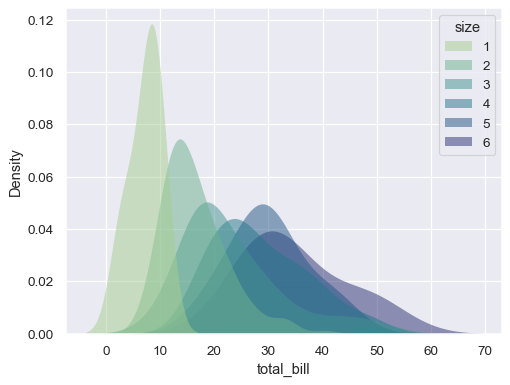
\includegraphics[width=0.6\textwidth]{images/kdeplot.png}
            \caption{Kernel density estimate (KDE) plot }%
            \label{fig:wust_logo}
        \end{figure}

    \section{Code}
    \code{Python}
\begin{lstlisting}
@staticmethod
def analyze_behavior_patterns(
    logs: list[dict], allowed_ids: list[str], logger: structlog.BoundLogger
) -> tuple[list[str], list[str]]:
    ...
    positive_tracks, negative_tracks = set(), set()

    for log in logs:
        if log["track_id"] in allowed_ids:
            if log["event"] == "NEXT" and float(log["percent"]) < 30:
                negative_tracks.add(log["track_id"])
            elif log["event"] == "PREVIOUS" and float(log["percent"]) > 70:
                positive_tracks.add(log["track_id"])
            elif float(log["percent"]) >= 90:
                positive_tracks.add(log["track_id"])

    return list(positive_tracks), list(negative_tracks)
\end{lstlisting}


% -------------------- References (from the references.bib file) --------------------
\bibliographystyle{plain}
\bibliography{references}
\end{document}

